\documentclass[14pt]{extarticle}
\usepackage[utf8]{inputenc}
\usepackage{tkz-euclide}
\usepackage{tikz} 
\usepackage{pdflscape}
\usepackage[margin=2cm]{geometry}
\usepackage{amsmath}
\usepackage{pgfplots}
\setlength\parindent{0pt}
\pgfplotsset{compat=1.16}  
\usetikzlibrary{arrows.meta}

\begin{document}
\begin{center}
    \LARGE{\textbf{Il piano cartesiano - Esercitazione 3}}
\end{center}
\vspace{1cm}

\begin{minipage}{0.7\textwidth}
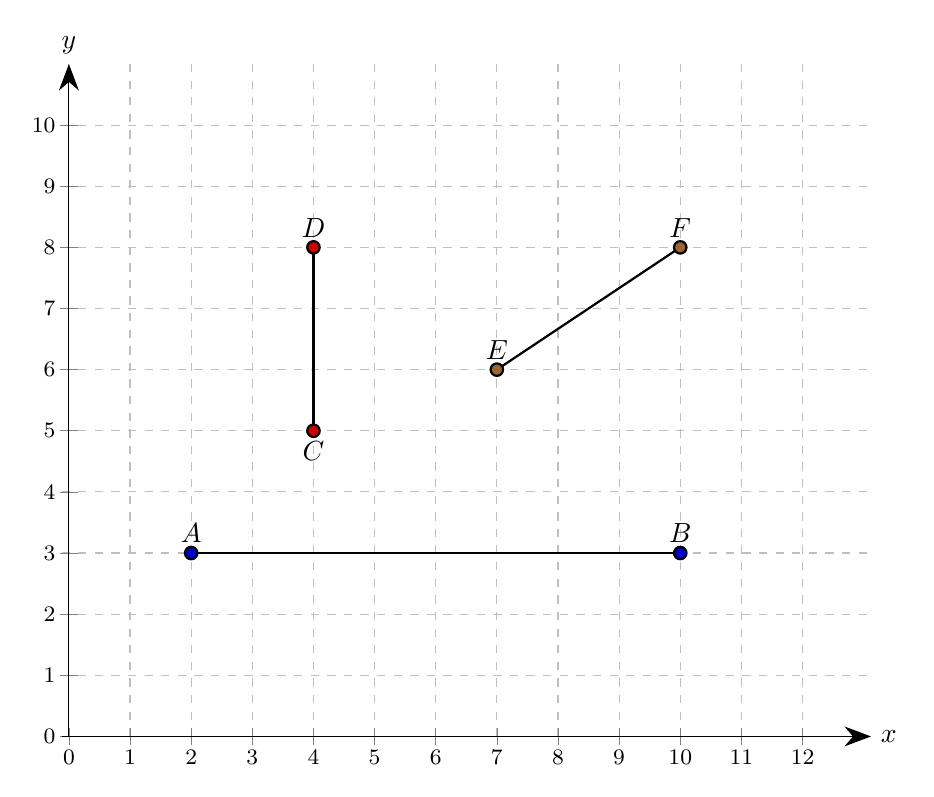
\begin{tikzpicture}[scale=1.5]
\begin{axis}[
    set layers,
    axis lines=middle,
    axis equal,
    %grid=both,
    grid, grid style=dashed,
    axis line style={-{Stealth[scale=2]}},
    xmax=11,
    ymax=11,
    xmin=2,
    ymin=0,
    xstep=1,
    ystep=1,
    xlabel=$x$, x label style={anchor=west}, 
    ylabel=$y$, y label style={anchor=south}, 
    ytick={0,...,10},
    xtick={0,...,12},
    extra y ticks={0},
    extra x ticks={0},
    ticklabel style={font=\footnotesize, fill=white, inner sep=1.5pt},
    mark size=1.5pt
    ]
\addplot+[color=black, thick=2,
      mark=*,
      ] coordinates{(2,3) (10,3)}
      node[pos=0,above] {$A$} node[pos=1,above] {$B$};
\addplot+[color=black, thick=2,
      mark=*,
      ] coordinates{(4,5) (4,8)}
      node[pos=0,below] {$C$} node[pos=1,above] {$D$};
\addplot+[color=black, thick=2,
      mark=*,
      ] coordinates{(7,6) (10,8)}
      node[pos=0,above] {$E$} node[pos=1,above] {$F$};
\end{axis}
\end{tikzpicture}
\end{minipage}
\begin{minipage}{0.3\textwidth}
    \(A(2;3)\)\\
    \(B(10;3)\)\\
    \(C(4;5)\)\\
    \(D(4;8)\)\\
    \(E(7;6)\)\\
    \(F(10;8)\)\\
\end{minipage}

\vspace{1cm}
Calcolo del segmento \(\overline{AB}\):
\[\overline{AB}=x_B-x_A\quad x_B>x_A\]
Calcolo del segmento \(\overline{CD}\):
\[\overline{CD}=y_D-y_C\quad y_D>y_C\]
Calcolo del segmento \(\overline{EG}\), si usa il Teorema di Pitagora:
\[\overline{EF}=\sqrt{(y_F-y_E)^2+(x_F-x_E)^2}\quad y_F>y_E \quad x_F>x_E\]


\clearpage
\textbf{Esercizio 1}: ricopia sul quaderno il grafico cartesiano, riporta i punti \(A\), \(B\), \(C\) e \(D\). Unisci i punti A-B,B-C,C-D e D-A, dimostra che l'area della figura ottenuta è uguale a quella di un quadrato di lato 1.\\
\begin{minipage}{0.7\textwidth}
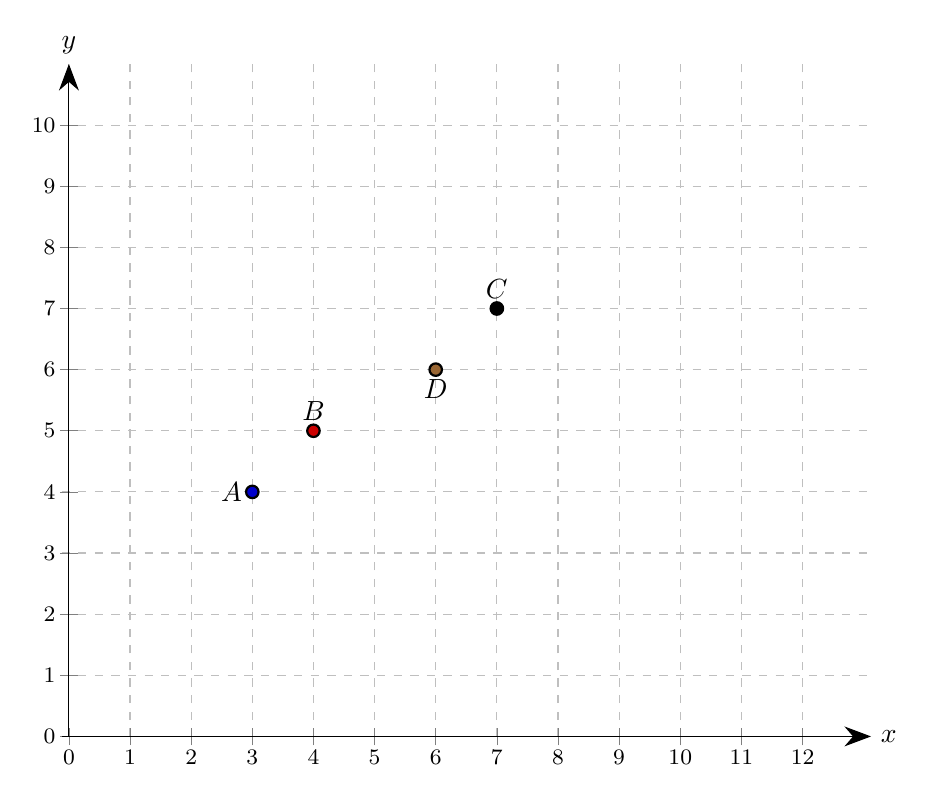
\begin{tikzpicture}[scale=1.5]
\begin{axis}[
    set layers,
    axis lines=middle,
    axis equal,
    %grid=both,
    grid, grid style=dashed,
    axis line style={-{Stealth[scale=2]}},
    xmax=11,
    ymax=11,
    xmin=2,
    ymin=0,
    xstep=1,
    ystep=1,
    xlabel=$x$, x label style={anchor=west}, 
    ylabel=$y$, y label style={anchor=south}, 
    ytick={0,...,10},
    xtick={0,...,12},
    extra y ticks={0},
    extra x ticks={0},
    ticklabel style={font=\footnotesize, fill=white, inner sep=1.5pt},
    mark size=1.5pt
    ]
\addplot+[color=black, thick=2,
      mark=*,
      ] coordinates{(3,4)}
      node[pos=0,left] {$A$};
\addplot+[color=black, thick=2,
      mark=*,
      ] coordinates{(4,5)}
      node[pos=0,above] {$B$};
\addplot+[color=black, thick=2,
      mark=*,
      ] coordinates{(6,6)}
      node[pos=0,below] {$D$};
\addplot+[color=black, thick=2,
      mark=*,
      ] coordinates{(7,7)}
      node[pos=0,above] {$C$};
\end{axis}
\end{tikzpicture}
\end{minipage}
\begin{minipage}{0.3\textwidth}
    \(A(3;4)\)\\
    \(B(4;5)\)\\
    \(C(7;7)\)\\
    \(D(6;6)\)\\
\end{minipage}
\vspace{1cm}

% \textbf{Esercizio 2}: ricopia sul quaderno il grafico cartesiano, indica le coordinate dei punti \(A\), \(B\), \(C\) e \(D\). Calcola perimetro ed area della figura ottenuta unendo i punti A-B,B-C,C-D e D-A.\\
% \begin{minipage}{0.7\textwidth}
% \begin{tikzpicture}[scale=1.5]
% \begin{axis}[
%     set layers,
%     axis lines=middle,
%     axis equal,
%     %grid=both,
%     grid, grid style=dashed,
%     axis line style={-{Stealth[scale=2]}},
%     xmax=11,
%     ymax=11,
%     xmin=2,
%     ymin=0,
%     xstep=1,
%     ystep=1,
%     xlabel=$x$, x label style={anchor=west}, 
%     ylabel=$y$, y label style={anchor=south}, 
%     ytick={0,...,10},
%     xtick={0,...,12},
%     extra y ticks={0},
%     extra x ticks={0},
%     ticklabel style={font=\footnotesize, fill=white, inner sep=1.5pt},
%     mark size=1.5pt
%     ]
% % \addplot+[color=black, thick=2,
% %       mark=*,
% %       ] coordinates{(6,2)}
% %       node[pos=0,above] {$A$};
% % \addplot+[color=black, thick=2,
% %       mark=*,
% %       ] coordinates{(2,2)}
% %       node[pos=0,above] {$B$};
% % \addplot+[color=black, thick=2,
% %       mark=*,
% %       ] coordinates{(2,8)}
% %       node[pos=0,above] {$C$};
% % \addplot+[color=black, thick=2,
% %       mark=*,
% %       ] coordinates{(6,8)}
% %       node[pos=0,above] {$D$};
% \end{axis}
% \end{tikzpicture}
% \end{minipage}
% \begin{minipage}{0.3\textwidth}
%     \(A(6;2)\)\\
%     \(B(2;2)\)\\
%     \(C(2;8)\)\\
%     \(D(6;8)\)\\
% \end{minipage}
% % \vspace{1cm}
% \clearpage
% \textbf{Esercizio 3}: ricopia sul quaderno il grafico cartesiano, indica le coordinate dei punti \(A\), \(B\), \(C\) e \(D\). Calcola perimetro ed area della figura ottenuta unendo i punti A-B,B-C,C-D e D-A.\\
% \begin{minipage}{0.7\textwidth}
% \begin{tikzpicture}[scale=1.5]
% \begin{axis}[
%     set layers,
%     axis lines=middle,
%     axis equal,
%     %grid=both,
%     grid, grid style=dashed,
%     axis line style={-{Stealth[scale=2]}},
%     xmax=11,
%     ymax=11,
%     xmin=2,
%     ymin=0,
%     xstep=1,
%     ystep=1,
%     xlabel=$x$, x label style={anchor=west}, 
%     ylabel=$y$, y label style={anchor=south}, 
%     ytick={0,...,10},
%     xtick={0,...,12},
%     extra y ticks={0},
%     extra x ticks={0},
%     ticklabel style={font=\footnotesize, fill=white, inner sep=1.5pt},
%     mark size=1.5pt
%     ]
% % \addplot+[color=black, thick=2,
% %       mark=*,
% %       ] coordinates{(6,2)}
% %       node[pos=0,above] {$A$};
% % \addplot+[color=black, thick=2,
% %       mark=*,
% %       ] coordinates{(2,2)}
% %       node[pos=0,above] {$B$};
% % \addplot+[color=black, thick=2,
% %       mark=*,
% %       ] coordinates{(4,6)}
% %       node[pos=0,above] {$C$};
% % \addplot+[color=black, thick=2,
% %       mark=*,
% %       ] coordinates{(8,6)}
% %       node[pos=0,above] {$D$};
% \end{axis}
% \end{tikzpicture}
% \end{minipage}
% \begin{minipage}{0.3\textwidth}
%     \(A(6;2)\)\\
%     \(B(2;2)\)\\
%     \(C(4;6)\)\\
%     \(D(8;6)\)\\
% \end{minipage}
% \vspace{0.7cm}
% % ---------- TRIANGOLO ---------------------

% % \textbf{Esercizio 3}: ricopia sul quaderno il grafico cartesiano, indica le coordinate dei punti \(A\), \(B\), \(C\) e \(D\). Unisci i punti A-B, B-C, C-A e calcola perimetro ed area della figura ottenutà. \\
% % \begin{minipage}{0.7\textwidth}
% % \begin{tikzpicture}[scale=1.5]
% % \begin{axis}[
% %     set layers,
% %     axis lines=middle,
% %     axis equal,
% %     %grid=both,
% %     grid, grid style=dashed,
% %     axis line style={-{Stealth[scale=2]}},
% %     xmax=11,
% %     ymax=11,
% %     xmin=2,
% %     ymin=0,
% %     xstep=1,
% %     ystep=1,
% %     xlabel=$x$, x label style={anchor=west}, 
% %     ylabel=$y$, y label style={anchor=south}, 
% %     ytick={0,...,10},
% %     xtick={0,...,12},
% %     extra y ticks={0},
% %     extra x ticks={0},
% %     ticklabel style={font=\footnotesize, fill=white, inner sep=1.5pt},
% %     mark size=1.5pt
% %     ]
% % \addplot+[color=black, thick=2,
% %       mark=*,
% %       ] coordinates{(10,2)}
% %       node[pos=0,above] {$A$};
% % \addplot+[color=black, thick=2,
% %       mark=*,
% %       ] coordinates{(4,2)}
% %       node[pos=0,above] {$B$};
% % \addplot+[color=black, thick=2,
% %       mark=*,
% %       ] coordinates{(7,5)}
% %       node[pos=0,above] {$C$};
% % \end{axis}
% % \end{tikzpicture}
% % \end{minipage}
% % \begin{minipage}{0.3\textwidth}
% %     \(A(10;2)\)\\
% %     \(B(4;2)\)\\
% %     \(C(7;5)\)\\
% % \end{minipage}
% % \vspace{1cm}

% %------- TEOREMA DI PITAGORA ---------
% \textbf{Esercizio 4}: Ricopia sul quaderno il grafico cartesiano e indica le coordinate dei punti \(A\), \(B\), \(C\), \(D\), \(E\), \(F\), \(G\), \(H\) e \(I\). Calcola l'area e il perimetro della figura.\\
% \begin{minipage}{0.7\textwidth}
% \begin{tikzpicture}[scale=1.5]
% \begin{axis}[
%     set layers,
%     axis lines=middle,
%     axis equal,
%     %grid=both,
%     grid, grid style=dashed,
%     axis line style={-{Stealth[scale=2]}},
%     xmax=12,
%     ymax=12,
%     xmin=2,
%     ymin=0,
%     xstep=1,
%     ystep=1,
%     xlabel=$x$, x label style={anchor=west}, 
%     ylabel=$y$, y label style={anchor=south}, 
%     ytick={0,...,11},
%     xtick={0,...,13},
%     extra y ticks={0},
%     extra x ticks={0},
%     ticklabel style={font=\footnotesize, fill=white, inner sep=1.5pt},
%     mark size=1.5pt
%     ]
% \addplot[color=black, thick=2,
%       mark=*,
%       ] coordinates{(7,5) (7,2)}
%       node[pos=0,right] {$B$};
% \addplot[color=black, thick=2,
%       mark=*,
%       ] coordinates{(4,5) (4,8) }
%       node[pos=0,below left] {$E$};
% % \addplot+[color=black, thick=2,
% %       mark=*,
% %       ] coordinates{(4,2) (4,5) }
% %       node[pos=0,below left] {$D$};
% \addplot[color=black, thick=2,
%       mark=*,
%       ] coordinates{(4,8) (7,5)}
%       node[pos=0,above] {$H$};
% \addplot[color=black, thick=2,
%       mark=*,
%       ] coordinates{(7,5) (4,5) };
% \addplot[color=black, thick=2,
%       mark=*,
%       ] coordinates{(7,2) (4,2)}
%       node[pos=0,below] {$C$}  node[pos=1,below] {$D$};
% \addplot[color=black, thick=2,
%       mark=*,
%       ] coordinates{(1,5) (1,8)}
%       node[pos=0,below] {$F$}  node[pos=1,above] {$G$};
% \addplot[color=black, thick=2,
%       mark=*,
%       ] coordinates{(7,11) (10,8)}
%       node[pos=0,above left ] {$I$}  node[pos=1,right ] {$A$};
% \addplot[color=black, thick=2,
%       mark=*,
%       ] coordinates{(4,8) (7,11)};
% \addplot[color=black, thick=2,
%       mark=*,
%       ] coordinates{(10,8) (7,5)};
% \addplot[color=black, thick=2,
%       mark=*,
%       ] coordinates{(4,2) (4,5)};
% \addplot[color=black, thick=2,
%       mark=*,
%       ] coordinates{(4,5) (1,5)};
% \addplot[color=black, thick=2,
%       mark=*,
%       ] coordinates{(4,8) (1,8)};
% \end{axis}
% \end{tikzpicture}
% \end{minipage}
% \begin{minipage}{0.3\textwidth}
%     \(A(?;?)\)\\
%     \(B(?;?)\)\\
%     \(C(?;?)\)\\
%     \(D(?;?)\)\\
%     \(E(?;?)\)\\
%     \(F(?;?)\)\\
%     \(G(?;?)\)\\
%     \(H(?;?)\)\\
%     \(I(?;?)\)\\
% \end{minipage}
% \vspace{1cm}


%\vspace{1cm}

% \textbf{Esercizio 3}: Ricopia sul quaderno il grafico cartesiano e indica le coordinate dei punti \(A\), \(B\), \(C\) e \(D\). Calcola l'area e il perimetro della figura.\\
% \begin{minipage}{0.7\textwidth}
% \begin{tikzpicture}[scale=1.5]
% \begin{axis}[
%     set layers,
%     axis lines=middle,
%     axis equal,
%     %grid=both,
%     grid, grid style=dashed,
%     axis line style={-{Stealth[scale=2]}},
%     xmax=11,
%     ymax=11,
%     xmin=2,
%     ymin=0,
%     xstep=1,
%     ystep=1,
%     xlabel=$x$, x label style={anchor=west}, 
%     ylabel=$y$, y label style={anchor=south}, 
%     ytick={0,...,10},
%     xtick={0,...,12},
%     extra y ticks={0},
%     extra x ticks={0},
%     ticklabel style={font=\footnotesize, fill=white, inner sep=1.5pt},
%     mark size=1.5pt
%     ]
% \addplot+[color=black, thick=2,
%       mark=*,
%       ] coordinates{(10,5) (10,1)}
%       node[pos=0,right] {$C$};
% \addplot+[color=black, thick=2,
%       mark=*,
%       ] coordinates{(4,5) (7,8) }
%       node[pos=0,above] {$B$};
% \addplot+[color=black, thick=2,
%       mark=*,
%       ] coordinates{(10,1) (4,5) }
%       node[pos=0,right] {$D$};
% \addplot+[color=black, thick=2,
%       mark=*,
%       ] coordinates{(7,8) (10,5)}
%       node[pos=0,above] {$A$};
% \addplot+[color=black, thick=2,
%       mark=*,
%       ] coordinates{(10,5) (4,5) };
% % \addplot+[color=black, thick=2,
% %       mark=*,
% %       ] coordinates{(10,1) (4,1)}
% %       node[pos=0,below] {$D$}  node[pos=1,below] {$E$};
% \end{axis}
% \end{tikzpicture}
% \end{minipage}
% \begin{minipage}{0.3\textwidth}
%     \(A(?;?)\)\\
%     \(B(?;?)\)\\
%     \(C(?;?)\)\\
%     \(D(?;?)\)\\
%     %\(E(?;?)\)\\
% \end{minipage}
% \vspace{1cm}

\end{document}